\subsection*{Question 4}

\textbf{a)} Answer the same question as in Q3 using a Metropolis algorithm with vector proposals for $\bm{\theta}$ and making use of the variance-covariance matrix from the Laplace approximation in Q2d. Use the same number of iterations (after burnin) as in Q3.

\begin{center}\rule{6cm}{0.4pt}\end{center}

In order to get $\SI{20}{\percent}$ of acceptance rate, we multiplied the variance obtained from the variance-covariance matrix by a factor of $20$.

\begin{figure}[H]
	\centering
	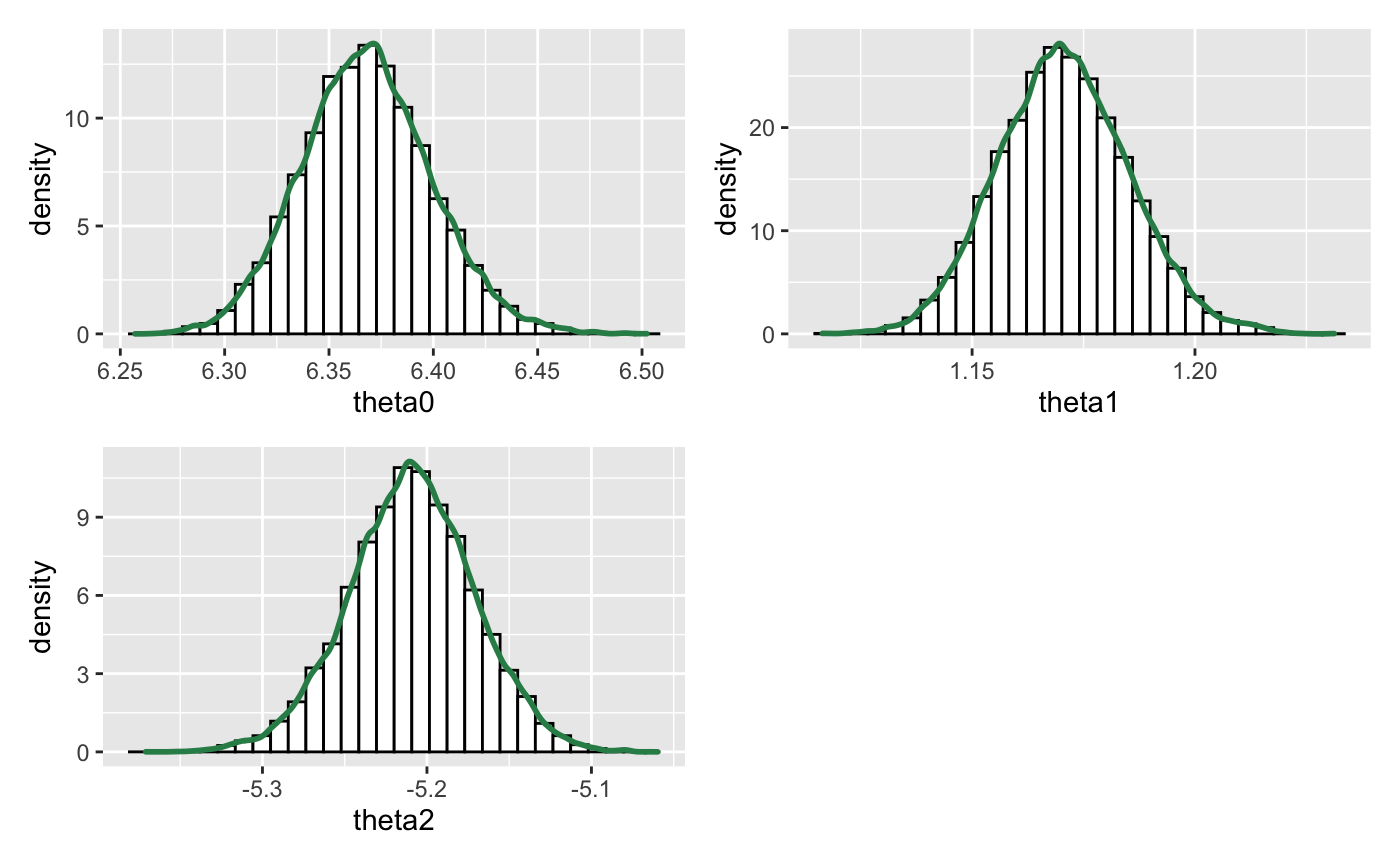
\includegraphics[width=0.7\textwidth]{figures/metropolis_vw_samples.png}
	\caption{Random sample from the posterior distribution of $(\vec{\theta}|\mathcal{D}_1)$ using a vector-wise metropolis algorithm}
	\label{fig:metropolis_vw_samples}
\end{figure}

\subsubsection*{Convergence}

\begin{figure}[H]
	\centering
	\begin{subfigure}{0.3\textwidth}
		\centering
		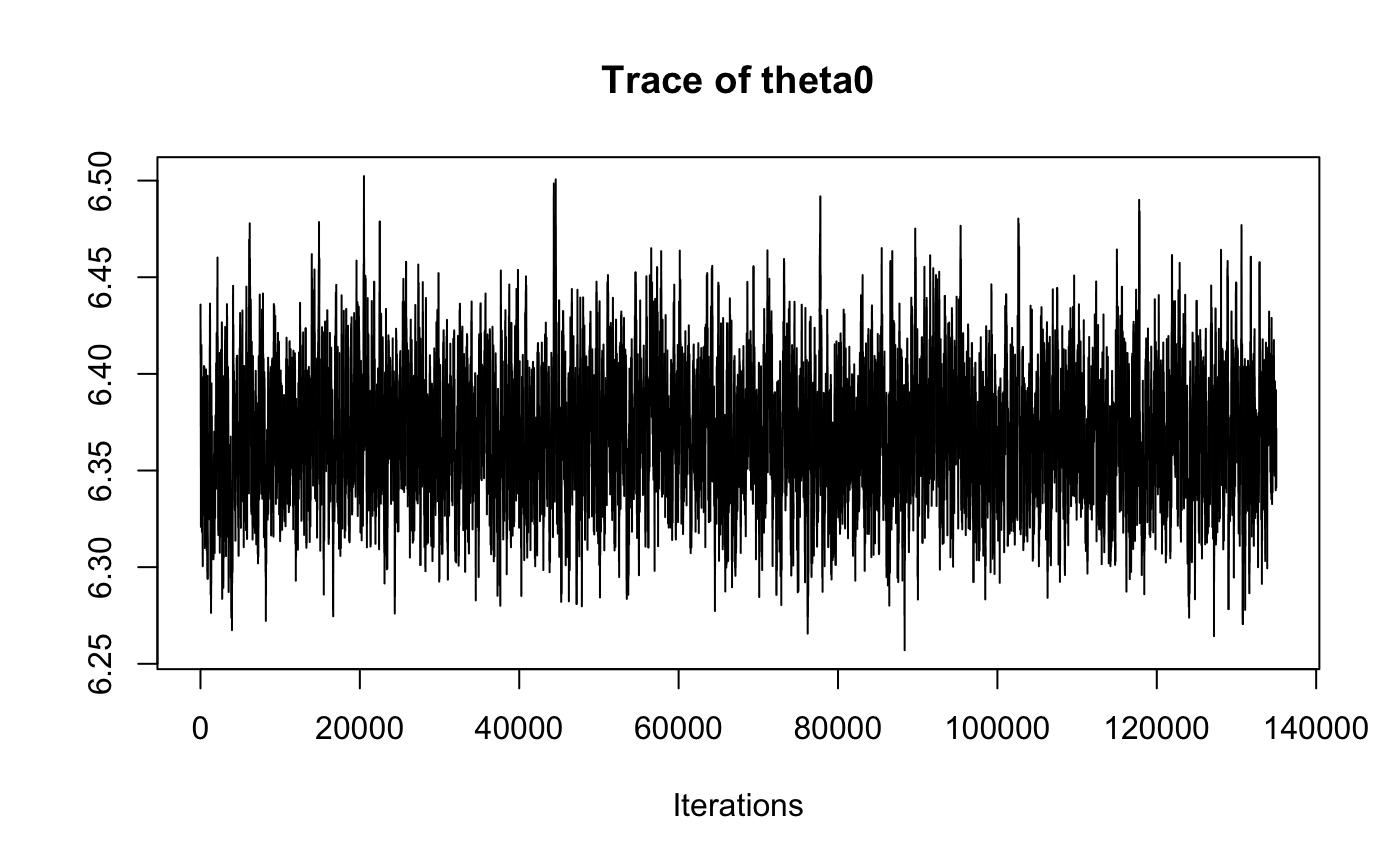
\includegraphics{figures/metropolis_vw_traceplot_theta0}
	\end{subfigure}
	\begin{subfigure}{0.3\textwidth}
		\centering
		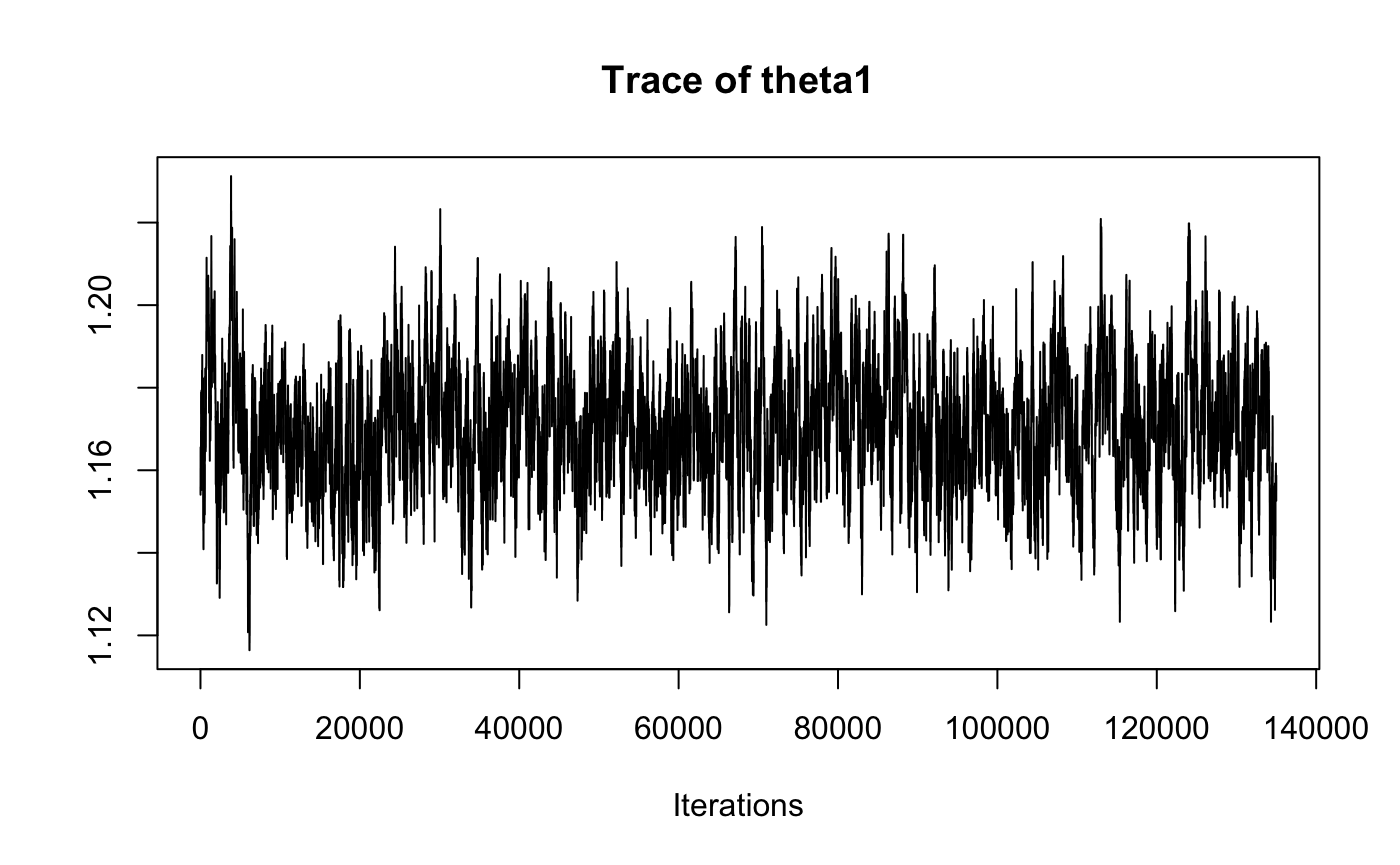
\includegraphics{figures/metropolis_vw_traceplot_theta1}
	\end{subfigure}
	\begin{subfigure}{0.3\textwidth}
		\centering
		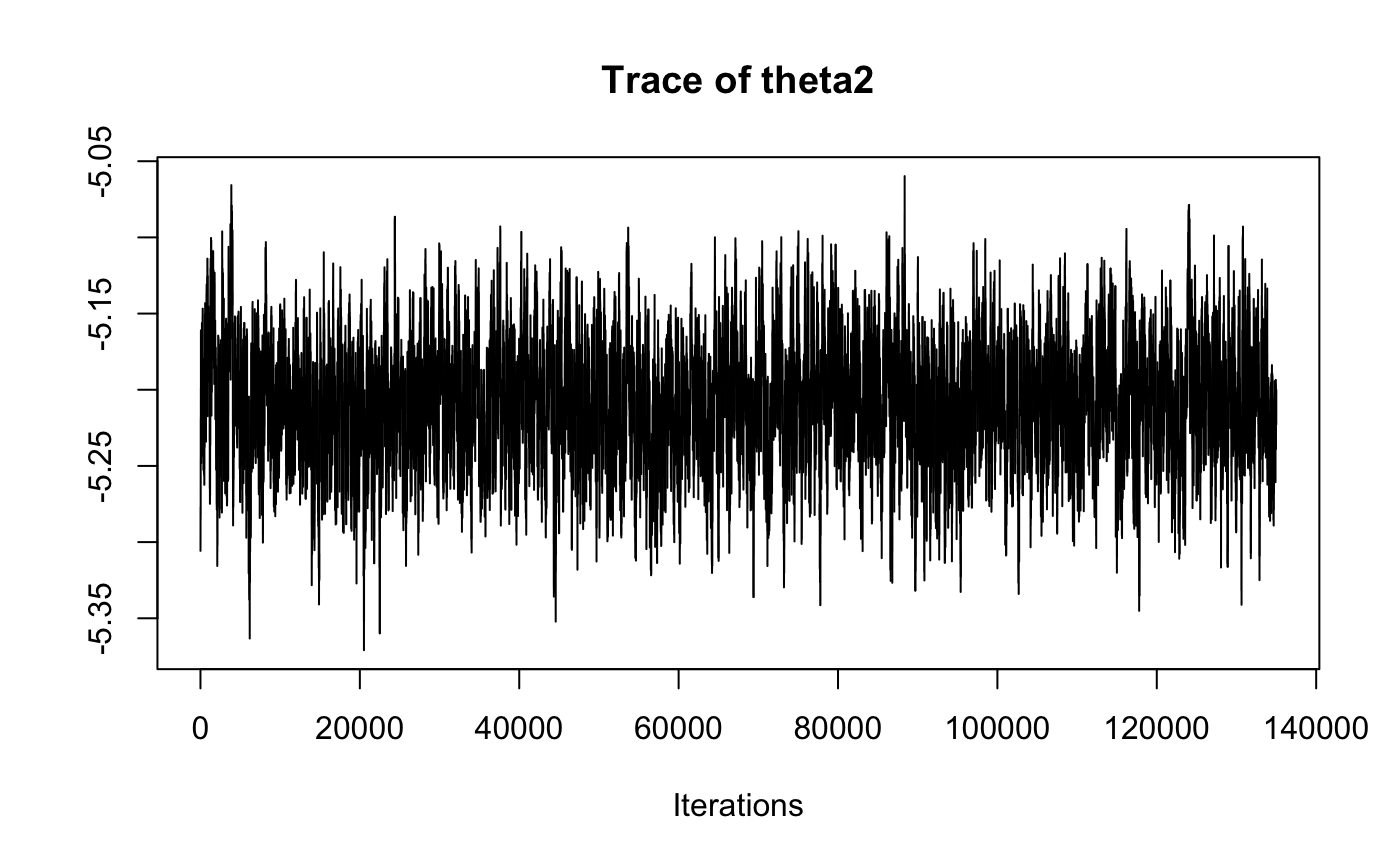
\includegraphics{figures/metropolis_vw_traceplot_theta2}
	\end{subfigure}
	\caption{Traceplots of the $\theta_k$ parameters}
	\label{fig:metropolis-vw-traceplots}
\end{figure}

\begin{table}[H]
	\centering\begin{tabular}{|c|c|c|} \hline 
		parameters & $\hat{R}$ & upper C.I. \\ \hline
		$\theta_0$ & $1.000833$ & $1.002573$ \\
		$\theta_1$ & $1.005029$ & $1.016367$ \\
		$\theta_2$ & $1.001695$ & $1.005931$ \\ \hline
	\end{tabular}
	\caption{Results of the Gelbman-Rubin test}
	\label{tab:metropolis-vw-gelman-rubin}
\end{table}

\begin{table}[H]
	\centering\begin{tabular}{|c|c|c|} \hline 
		$\theta_0$ & $\theta_1$ & $\theta_2$ \\ \hline 
		$-1.1272$   &   $-0.1770$	&   $0.7131$ \\ \hline
	\end{tabular}
	\caption{Results for the Geweke statistic (z-score)}
	\label{tab:metropolis-cw-geweke}
\end{table}

\textbf{b)} Compare your results with the previous ones.

\begin{center}\rule{6cm}{0.4pt}\end{center}

\subsubsection*{Effective sample size}

\begin{table}[H]
	\centering\begin{tabular}{|c|c|c|} \hline 
		$\theta_0$ & $\theta_1$ & $\theta_2$ \\ \hline 
		$1550.8856$  & $495.6665$ & $1225.5307$   \\ \hline
	\end{tabular}
	\caption{Effective sample sizes}
	\label{tab:metropolis-vw-effective-sample-sizes}
\end{table}

\subsubsection*{Fitted curve}

\begin{figure}[H]
	\centering
	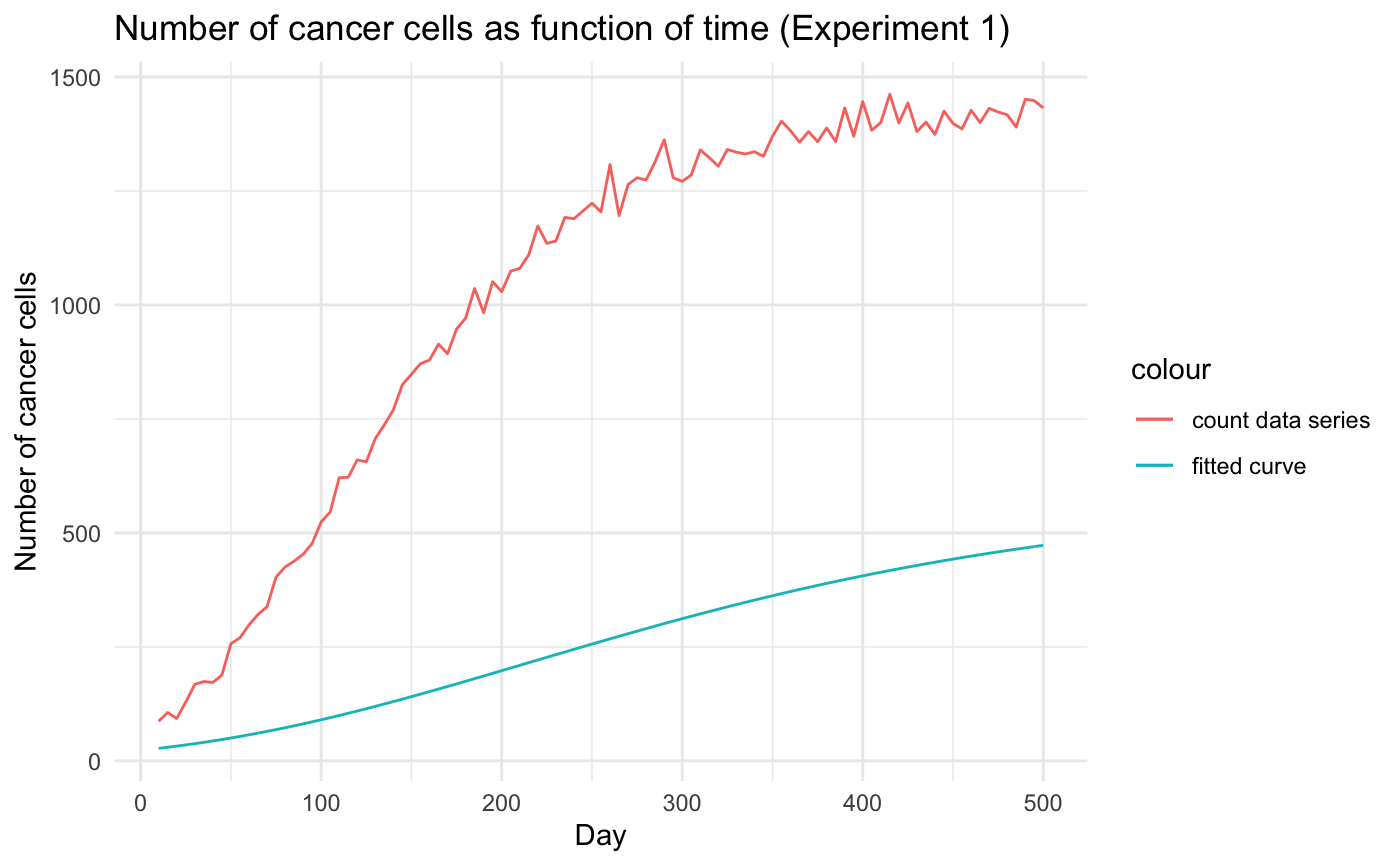
\includegraphics[width=0.7\textwidth]{figures/metropolis_vw_fitted_curve.png}
	\caption{Comparison of the observed count data series for experiment 1 (\textit{black}) with the fitted curve for $\mu(t)$ (\textit{red})}
	\label{fig:metropolis-vw-fitted-curve}
\end{figure}

\subsubsection*{Point estimate and $\SI{95}{\percent}$ credible region}

\begin{table}[H]
	\centering\begin{tabular}{|c|c|c|} \hline 
		Parameter & Median & Mean \\ \hline 
		$\theta_0$ & $6.37$ & $6.37$ \\ 
		$\theta_1$ & $1.17$ & $1.17$ \\
		$\theta_2$ & $-5.21$ & $-5.21$ \\ \hline
	\end{tabular}
	\caption{Point estimates of $\bm{\theta}$ parameters}
	\label{tab:metropolis-cw-point-estimates}
\end{table}

\begin{table}[H]
	\centering\begin{tabular}{|c|c|c|} \hline 
		Parameter & Lower & Upper \\ \hline 
		$\theta_0$ & $6.31$ & $6.42$ \\ 
		$\theta_1$ & $1.14$ & $1.19$ \\
		$\theta_2$ & $-5.28$ & $-5.13$ \\ \hline
	\end{tabular}
	\caption{$\SI{95}{\percent}$ credible region for $\bm{\theta}$ parameters}
	\label{tab:metropolis-cw-credible-region}
\end{table}